\section{Validation Protocol and Simulation Results}
\label{sec:valid}
\subsection{Evidence and Performance Definitions}
The authoritative comparison, generated on 15 November 2026, contains $432$ simulated trials: three controller labels, twelve scenarios, and twelve seeds ($3000$--$3011$). Each trial lasts $60\,\mathrm s$. Initial range is sampled uniformly from $d^\ast+[0.25,0.45]\,\mathrm m$, bearing from $[-15^\circ,15^\circ]$, and relative heading from $[-5^\circ,5^\circ]$. The same scenario and seed schedule is used for each method. Saved configurations, source snapshots, hashes, per-trial metrics, and seed-$3000$ traces identify the evaluated implementation. A separate sensitivity study contains $78$ trials with seeds $4000$--$4005$.

\textbf{All closed-loop results in this section are synthetic.} The acoustic generator and estimator share the same response family, except for the specified perturbations. The trials assess implementation behavior under stated assumptions; they cannot validate the actual horn response or room acoustics. The $26$ saved Python tests cover model calculations, calibration rejection, protocol handling, delayed correction, supervision, and software motor-heartbeat behavior. They do not exercise physical motors or ADC acquisition.

Let $e_i=\rho_i-d^\ast$ and let $\mathcal T$ contain the last ten seconds of a run. Reported tail metrics are
\begin{equation}
\bar e=\frac{1}{|\mathcal T|}\sum_{i\in\mathcal T}e_i,\quad
e_{\mathrm{RMS}}=\sqrt{\frac{1}{|\mathcal T|}\sum_{i\in\mathcal T}e_i^2},
\end{equation}
and the analogous bearing RMS. A practical tracking pass requires $|\bar e|\le0.15\,\mathrm m$, bearing RMS $\le10^\circ$, TRACK occupancy at least $70\%$ over the full trial, and no simulated clearance violation. The mean-error gate is not an RMSE gate: a run can meet it despite substantial fluctuations. Aggregated RMSE includes every seed, including failed trials.

The original transient objective is retained separately: $2\%$ settling within $6\,\mathrm s$ and overshoot at most $15\%$. The saved implementation defines the settling band as $0.02|e_0|$, requires all subsequent samples to remain inside it, and measures time from trial start, including acquisition. For the positive initial errors used here, overshoot is $100\max\{0,-\min_i e_i\}/|e_0|$. No post-step time origin is introduced for the speed-change scenario. This convention is strict under noise and should not be confused with a fitted dominant-pole settling estimate.

\begin{table*}[t]
\centering\footnotesize
\caption{Controller comparison over twelve seeds per scenario. Each cell gives practical tracking passes / mean tail range RMSE in metres. All outcomes, including failures, enter the mean.}
\label{tab:comparison}
\begin{tabular}{@{}lccc@{}}\toprule
Scenario & LQI & Pole placement & Bearing-only steering\\\midrule
Nominal following & 12/12 / 0.0041 & 12/12 / 0.0043 & 0/12 / 0.1697 \\
Target speed increase & 12/12 / 0.0041 & 12/12 / 0.0043 & 0/12 / 0.2651 \\
Gentle turn & 12/12 / 0.0044 & 12/12 / 0.0045 & 0/12 / 0.1698 \\
Actuator mismatch & 12/12 / 0.0036 & 12/12 / 0.0038 & 0/12 / 0.8086 \\
Five-second signal loss & 12/12 / 0.0043 & 12/12 / 0.0044 & 1/12 / 0.1577 \\
Noise, drops, amplitude outliers, jitter & 11/12 / 0.1210 & 11/12 / 0.1206 & 10/12 / 0.7447 \\
Source gain $+20\%$ & 0/12 / 0.2412 & 0/12 / 0.2413 & 12/12 / 0.0363 \\

\bottomrule\end{tabular}
\end{table*}

\subsection{Regulation and Disturbance Response}
Both integral controllers pass all twelve nominal straight-following trials, the $0.05\,\mathrm{m/s}$ target-speed increase at $20\,\mathrm s$, the gentle turn, the actuator mismatch, and the five-second signal outage. The turn applies target yaw rate $0.025\,\mathrm{rad/s}$ between $15$ and $40\,\mathrm s$; actuator mismatch scales realized speed by $0.8$ and both lag constants by $1.7$. These perturbations are selected test conditions, not estimated physical distributions.

Nominal LQI mean tail range RMSE is $0.00409\,\mathrm m$, with worst-seed bearing RMS $0.545^\circ$. The constant-speed baseline passes none of the nominal trials and has mean tail range RMSE $0.170\,\mathrm m$. Its small bearing error does not imply distance regulation. Pole placement produces similar tracking outcomes to LQI; the present experiment supports both designs and does not establish statistical superiority of either.

\begin{figure*}[t]
\centering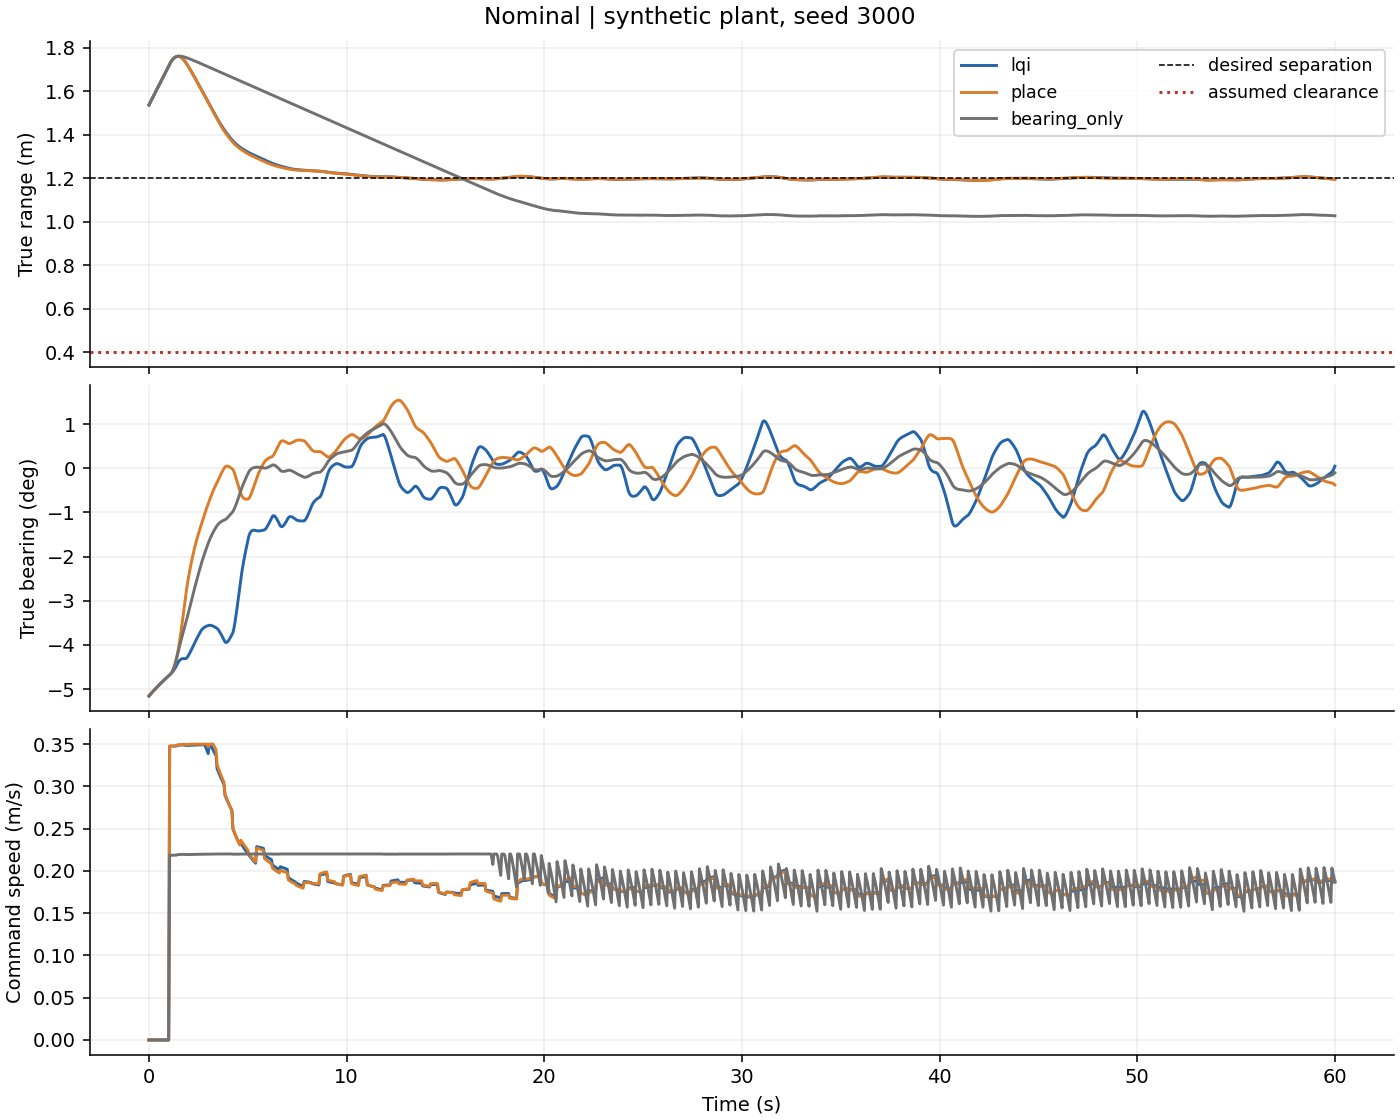
\includegraphics[width=0.88\textwidth]{figures/nominal.png}
\caption{Nominal synthetic response for seed $3000$, copied from the authoritative comparison run. The twelve-seed aggregates, rather than this example trace alone, determine reported pass counts.}
\label{fig:nominal}
\end{figure*}

In the combined stress case, additive amplitude noise doubles, packet-drop probability is $0.15$, independent amplitude perturbations occur on $12\%$ of pairs, and requested pair intervals vary by up to $15\%$. The amplitude perturbation is a synthetic reflection proxy, not a wave-propagation model. LQI and pole placement each pass $11/12$ trials; LQI mean tail range RMSE is $0.121\,\mathrm m$ and worst-seed bearing RMS is $3.11^\circ$. The baseline passes $10/12$ by the mean-error criterion but has mean RMSE $0.745\,\mathrm m$, illustrating why pass counts alone are insufficient.

The outage from $18$ to $23\,\mathrm s$ forces stopping and subsequent stationary reacquisition. Both integral designs recover under the modeled conditions. Neither result removes the need to measure loss-detection and motor-stop latency.

\begin{figure*}[t]
\centering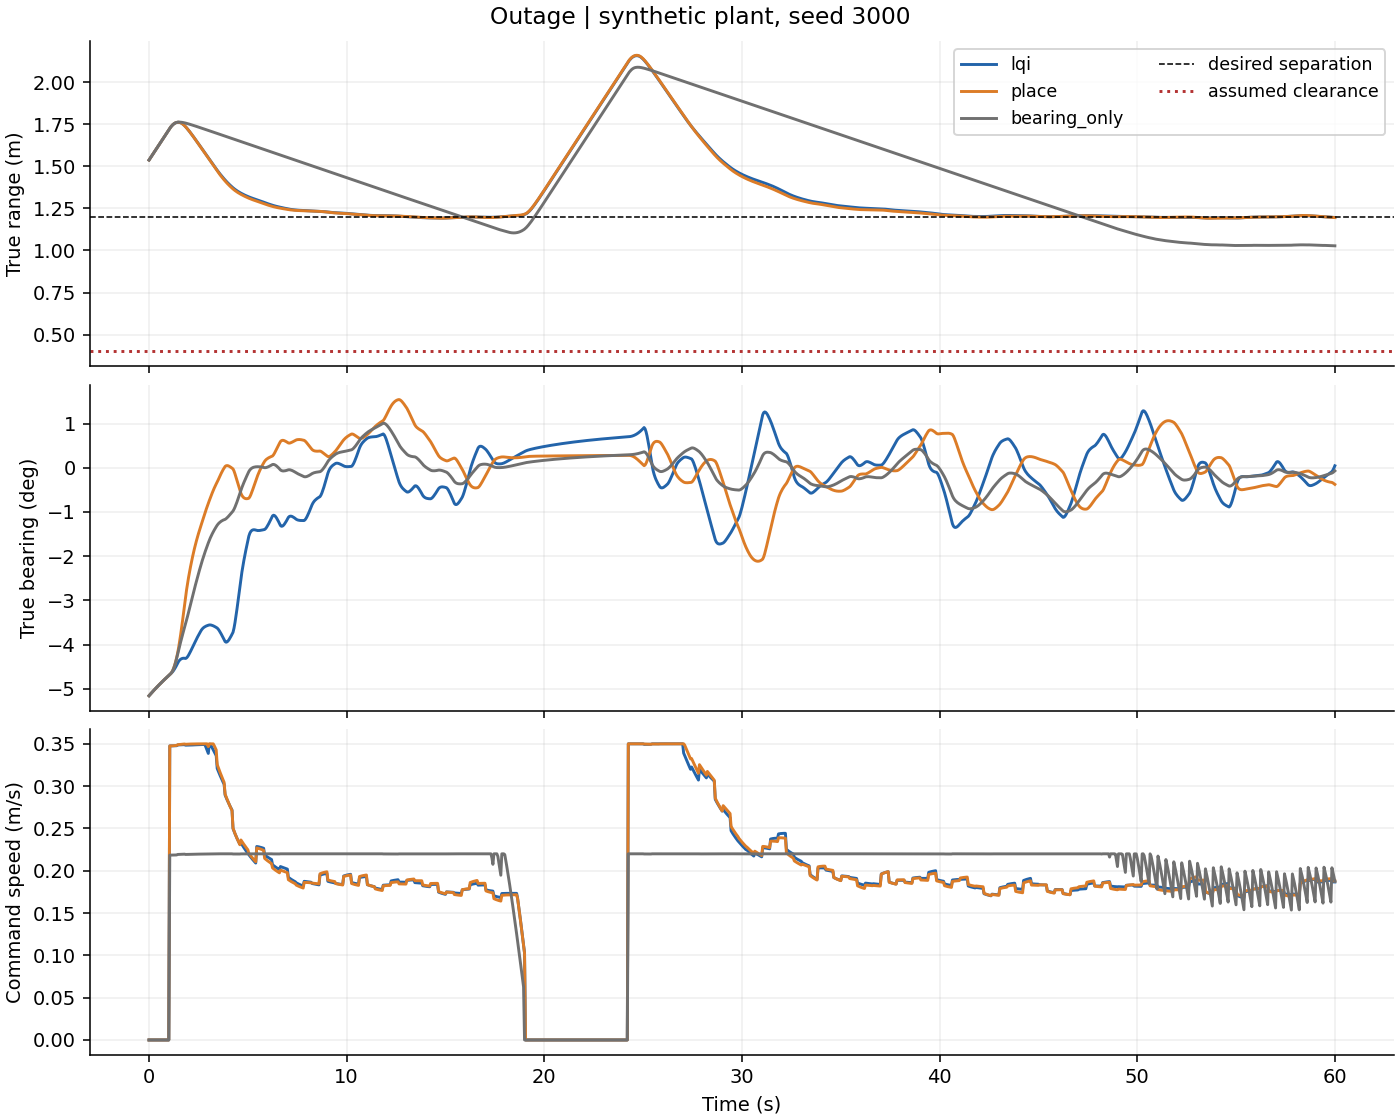
\includegraphics[width=0.88\textwidth]{figures/outage.png}
\caption{Synthetic five-second signal interruption, seed $3000$. State estimates, commands, and vehicle response are evaluated with the acquisition/hold logic active.}
\label{fig:outage}
\end{figure*}

\subsection{Failure Cases and Separate Terminal Tests}
A common source-level increase of $20\%$ produces LQI tail range RMSE $0.241\,\mathrm m$ and zero practical tracking passes. With $n=1$, Eq.~\eqref{eq:gainbias} predicts a true equilibrium shift of $0.2d^\ast=0.24\,\mathrm m$, consistent with the simulation. Integral action regulates the biased estimate. The baseline's $12/12$ passes in this single biased scenario result from its shared constraints and particular trajectory; they do not demonstrate rejection of arbitrary gain drift.

No-source trials and the $1.2\,\mathrm s$ and $12.84\,\mathrm s$ pair-period cases command zero motion in all twelve LQI trials. These are successful motion-inhibition tests, not tracking successes. A target at $0.50\,\mathrm{m/s}$ exceeds the follower's configured $0.35\,\mathrm{m/s}$ speed limit and cannot be followed at the desired separation. Its tracking failures are retained.

The explicitly declared stationary-source mission passes its separate standoff metric in $12/12$ trials under each controller label. This metric checks final-ten-second absolute mean range error at most $0.15\,\mathrm m$ and clearance; it does not independently test stop-latch activation. For LQI-labeled runs, mean final-ten-second range error is approximately $+0.060\,\mathrm m$, worst bearing RMS is $2.74^\circ$, and minimum range is $1.243\,\mathrm m$. These results concern the shared proportional terminal controller. Stop-latch behavior must also be checked in the command/mode history. Applying the moving-tracking occupancy criterion would incorrectly penalize an intended final stop.

No configured clearance violation occurs in the $432$ comparison trials or the $78$ sensitivity trials. This statement refers only to the modeled reference-point clearance. It is not an experimental collision-avoidance guarantee.

\subsection{Sensitivity to Measurement Assumptions}
With correct calibration in both generator and estimator, increasing Gaussian width $\sigma$ from $25^\circ$ to $160^\circ$ increases worst-seed tail bearing RMS from $0.329^\circ$ to $7.44^\circ$; all six trials at each width pass. A broad response reduces differential amplitude information. This sweep tests sensitivity under the assumed amplitude level, not the actual horn's shape or available signal-to-noise ratio.

Requested capture gaps of $0.10$, $0.18$, and $0.30\,\mathrm s$ pass six trials each. A $0.50\,\mathrm s$ gap with a $1.0\,\mathrm s$ pair period fails all six, with mean tail range RMSE approximately $0.177\,\mathrm m$. Raising control frequency cannot undo within-pair motion error. Additive amplitude-noise sweeps from $0.2$ to $5$ counts pass under the assumed $K=100$ amplitude calibration; these absolute noise values are not transferable to another gain setting.

\subsection{Robustness Analysis and Unmet Objectives}
A separate local periodic reference includes actuator lag, intermittent linear-observer corrections, exact delayed replay, and an Euler integral state. Its monodromy matrix is the product of the step maps over one measurement period; local stability requires every eigenvalue to lie inside the unit circle. The tested periods are $\{0.2,0.4,0.8,1.2\}\,\mathrm s$, delays $\{0,0.1,0.3\}\,\mathrm s$, and feedback-gain multipliers $\{0.5,1,2\}$. All $33$ valid combinations with delay shorter than the period are stable; the remaining three combinations are excluded by the reference formulation.

This reference assumes known realized actuator forcing in the predictor and exact replay. Its weak sensitivity to delay is conditional on those assumptions. The runtime uses modeled own motion and nonlinear measurements, and can fail an acquisition or performance criterion even when the local periodic reference is stable. The sweep does not establish the progress report's proposed $45^\circ$ phase margin or $6\,\mathrm{dB}$ gain margin.

The current LQI tuning meets the original joint settling/overshoot target in none of the nominal trials. The practical tail criterion is an explicitly revised commissioning metric, not evidence that the original transient target was achieved. Physical tuning and any revised specification must be justified using measured sensing delay, noise, motor deadband, and steering authority.

\begin{table}[t]
\caption{Disposition of the progress-report objectives.}
\label{tab:spec}\centering\footnotesize
\begin{tabularx}{\columnwidth}{@{}lX@{}}\toprule
ID & Current interpretation and evidence\\\midrule
O1 & Integral rejection of constant speed mismatch is local and conditional on calibration and feasible actuation; true-range bias persists under gain error.\\
O2 & Original bearing RMS limits: $10^\circ$ stationary, $20^\circ$ moving. The practical simulation gate uses the stricter $10^\circ$ moving limit.\\
O3 & Original $2\%$ settling $\le6\,\mathrm s$ and overshoot $\le15\%$: not achieved jointly by nominal LQI.\\
O4 & Configured limits and clearance checked in simulation. Physical stopping and clearance remain unverified.\\
O5 & Periodic local stability sweep completed. Original $45^\circ$ phase / $6\,\mathrm{dB}$ gain margins remain unverified.\\\bottomrule
\end{tabularx}
\end{table}

\pending{V1 --- Final robustness and transient claims}{After physical identification, rerun the simulations with the measured configuration; report original O1--O5 outcomes, transient distributions and failures. If classical margins are retained, define the loop break, delayed linearized model and treatment of the other channel. Otherwise explicitly revise the robustness objective.}
